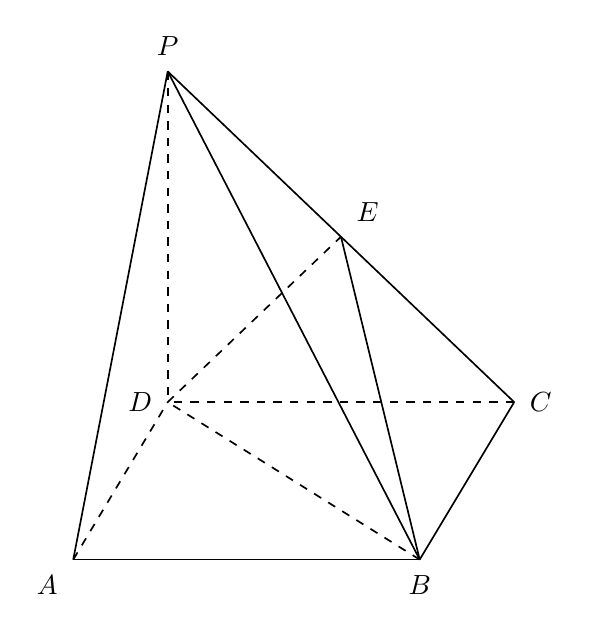
\begin{tikzpicture}[line width=0.6pt, font=\normalsize, >=stealth]
% P-ABCD 阳马: PD⊥底面, E为PC中点, EB竖直
\coordinate (P) at (-2,5);
\coordinate (D) at (-2,0.8);
\coordinate (A) at (-3.2,-1.2);
\coordinate (B) at (1.2,-1.2);
\coordinate (C) at (2.4,0.8);
\coordinate (E) at (0.2,2.9);
% 实线: 轮廓与可见棱
\draw[black] (P) -- (A);
\draw[black] (P) -- (B);
\draw[black] (P) -- (E);
\draw[black] (E) -- (C);
\draw[black] (A) -- (B);
\draw[black] (B) -- (C);
\draw[black] (B) -- (E);
% 虚线: 遮挡棱
\draw[black, dashed] (P) -- (D);
\draw[black, dashed] (A) -- (D);
\draw[black, dashed] (B) -- (D);
\draw[black, dashed] (C) -- (D);
\draw[black, dashed] (D) -- (E);
% 标签(避碰偏移)
\node[above=2pt] at (P) {$P$};
\node[left=2pt] at (D) {$D$};
\node[below left=2pt] at (A) {$A$};
\node[below=2pt] at (B) {$B$};
\node[right=2pt] at (C) {$C$};
\node[above right=2pt] at (E) {$E$};
\end{tikzpicture}
